\documentclass[
	letterpaper,
	a4paper,
	cleardoublepage=empty,
	headings=twolinechapter,
	numbers=autoenddot,
]{report}

\usepackage[a4paper, total={6in, 8in}]{geometry}

\usepackage{amsmath}
\usepackage{amsfonts}
\usepackage{amssymb}
\usepackage{tikz}
\usepackage{epigraph}
\usepackage{import}
\usepackage{float}

\usepackage{graphicx}
\usepackage{caption}
\usepackage{subcaption}

\usepackage{todonotes}
\usepackage{verbatim}

\usepackage{siunitx}

\newcommand{\Fig}[0]{Fig.}
\newcommand{\Eq}[0]{Eq.}

\newcommand\mykern{\ifmmode\kern0pt\else\kern0.08em\fi}
\renewcommand\epigraphflush{flushright}
\renewcommand\epigraphsize{\normalsize}
\setlength\epigraphwidth{0.7\textwidth}

\definecolor{titlepagecolor}{cmyk}{1,.60,0,.40}

\DeclareFixedFont{\titlefont}{T1}{ppl}{b}{it}{0.3in}
\DeclareSIPrefix{\femto}{f\mykern}{-15}

\makeatletter                       
\def\printauthor{%                  
	{\large \@author}}              
\makeatother
\author{
	3649361 - Wasim Essbai
	3638165 - Krutath Patel
	3640881 - Bhushan Bhad
	3637933 - Himanshu Duvedi
}
\newcommand\titlepagedecoration{%
	\begin{tikzpicture}[remember picture,overlay,shorten >= -10pt]
		
		\coordinate (aux1) at ([yshift=-15pt]current page.north east);
		\coordinate (aux2) at ([yshift=-410pt]current page.north east);
		\coordinate (aux3) at ([xshift=-4.5cm]current page.north east);
		\coordinate (aux4) at ([yshift=-150pt]current page.north east);
		
		\begin{scope}[titlepagecolor!40,line width=12pt,rounded corners=12pt]
			\draw
			(aux1) -- coordinate (a)
			++(225:5) --
			++(-45:5.1) coordinate (b);
			\draw[shorten <= -10pt]
			(aux3) --
			(a) --
			(aux1);
			\draw[opacity=0.6,titlepagecolor,shorten <= -10pt]
			(b) --
			++(225:2.2) --
			++(-45:2.2);
		\end{scope}
		\draw[titlepagecolor,line width=8pt,rounded corners=8pt,shorten <= -10pt]
		(aux4) --
		++(225:0.8) --
		++(-45:0.8);
		\begin{scope}[titlepagecolor!70,line width=6pt,rounded corners=8pt]
			\draw[shorten <= -10pt]
			(aux2) --
			++(225:3) coordinate[pos=0.45] (c) --
			++(-45:3.1);
			\draw
			(aux2) --
			(c) --
			++(135:2.5) --
			++(45:2.5) --
			++(-45:2.5) coordinate[pos=0.3] (d);   
			\draw 
			(d) -- +(45:1);
		\end{scope}
	\end{tikzpicture}%
}

\begin{document}
	\pagenumbering{roman}
	\begin{titlepage}
		
		\noindent
		\titlefont A Digital Readout Technique for \par Capacitive Sensor Applications\par
		\epigraph{Seminar Group IIC: Paper no. 15}
		\null\vfill
		\vspace*{1cm}
		\noindent
		\hfill
		\begin{minipage}{0.35\linewidth}
			\begin{flushright}
				\printauthor
			\end{flushright}
		\end{minipage}
		%
		\begin{minipage}{0.02\linewidth}
			\rule{1pt}{125pt}
		\end{minipage}
		\titlepagedecoration
	\end{titlepage}

	\tableofcontents
	\pagebreak
	
	\cleardoublepage
	\pagenumbering{arabic}
	
	\section*{Introduction}
	\addcontentsline{toc}{chapter}{Introduction}
	
	In this article, a technique for capacitance measurement is discussed, based on the work of Kung et al.\cite{Kung1988}. The technique is an particular implementation of the charge redistribution method \cite{4314753}.

	The presented approach gives a digital output, that could be converted to analog by a DAC(\textit{Digital to Analog Converter}) for further processings. This technique allows to reach high measurment resolution since it deletes errors due to: Parasitic capacitances, op-amp offset or charge injection from MOS switch. In figure \Fig~\ref{fig:CompleteCircuit} is showed the circuit that performs the described functions.
	\begin{figure}[h]
		\centering
		\begin{subfigure}{.5\textwidth}
			\centering
			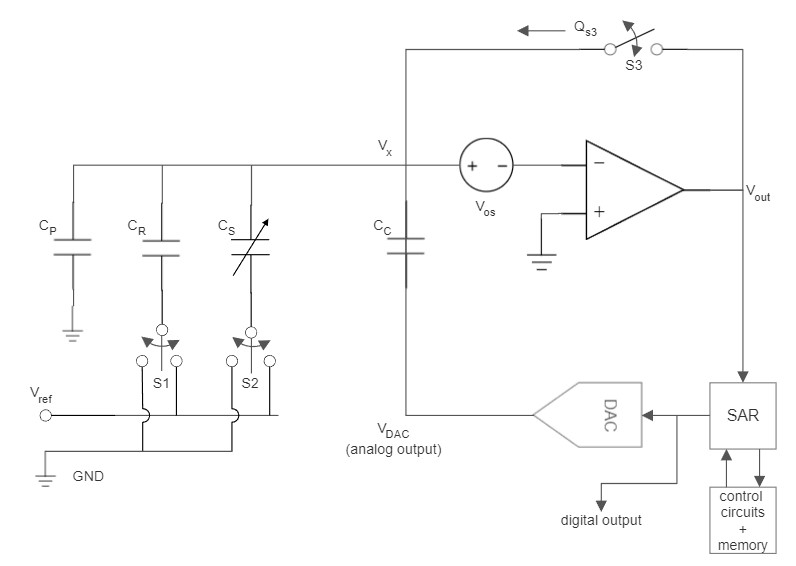
\includegraphics[width=0.6\linewidth]{ImageFiles/CompleteCircuit}
			\caption{Capacitance measurement circuit.}
			\label{fig:CompleteCircuit}
		\end{subfigure}%
		\begin{subfigure}{.5\textwidth}
			\centering
			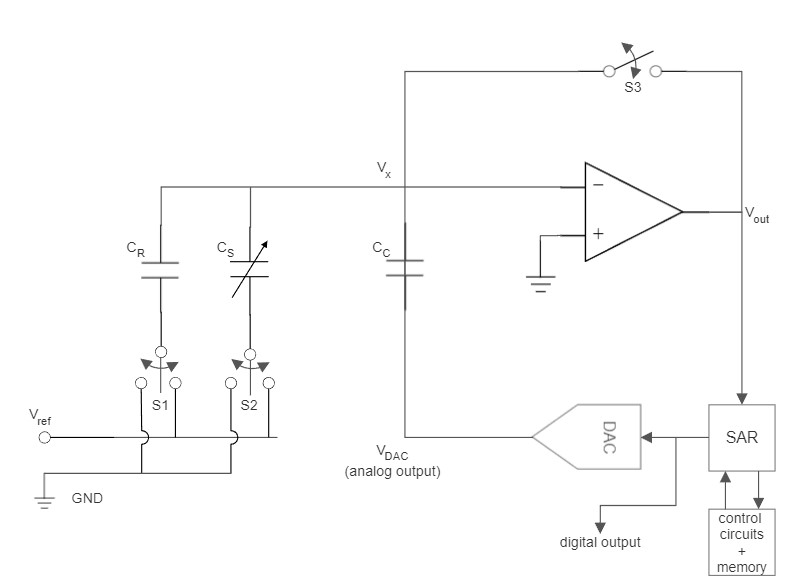
\includegraphics[width=0.6\linewidth]{ImageFiles/IdealCircuit}
			\caption{Capacitance measurement circuit without nonidealities.}
			\label{fig:IdealCircuit}
		\end{subfigure}
	\end{figure}
	\section*{Ideal Analysis}
	\addcontentsline{toc}{chapter}{Ideal Analysis}
	
	\import{./TextFiles/}{ideal_analysis.tex}
	
	\section*{Non Ideal Analysis}
	\addcontentsline{toc}{chapter}{Non Ideal Analysis}
	
	\import{./TextFiles/}{non_ideal_analysis.tex}
		
	\section*{Conclusions}
	\addcontentsline{toc}{chapter}{Conclusion}	
	
	It has been demonstrated that this technique can measure capacitance differences with a resolution of \SI{0.05}{\femto\farad} on capacitors in the 20-100 \si{\femto\farad} range, with parasitic capacitances around 100 times larger\cite{Kung1988}. The significant nonideal effects can be corrected through calibration. Furthermore, digital averaging can improve resolution, but at the cost of longer measurement times.
	
	This is a simple circuit and inherently compatible with digital signal processing. This makes it hightly suited for capacitance difference measurement in digital systems.
	
	\bibliographystyle{ieeetr}
	
	\bibliography{./OtherFiles/Bibliography}
	
	\addcontentsline{toc}{chapter}{Bibliography}
\end{document}